


%%%%%%%%%%%%%%%%%%%%%%%%%%%%%%%%%%%%%%%%%%%%%%%%%%%%%%%%%%%%%%%%%%%%%%%%
\chapter{Introduction}
%%%%%%%%%%%%%%%%%%%%%%%%%%%%%%%%%%%%%%%%%%%%%%%%%%%%%%%%%%%%%%%%%%%%%%%%


MacSim is a heterogeneous architecture simulator, specifically
supporting x86 ISA and NVIDIA PTX ISA. It is a trace-driven
cycle-level simulator.  It can simulate homogeneous ISA multicore
simulations, heterogeneous ISA multicore simulations. It uses
GPUOcelot~\cite{ocelot} for PTX trace generation and Pin~\cite{pin} to
generate x86 traces. Both traces are converted internal RISC style
uops and those uops are simulated. MacSim is a microarchitecture
simulator that simulates detailed pipeline (in-order and out-of-order)
and a memory system including caches, NoC, memory controllers. It
supports, asymmetric multicore configurations (small cores + medium
cores + big cores) and SMT or MT architectures as well.

Currently interconnection network model (based on IRIS) and power
model (based on McPat~\cite{mcpat}) are connected. ARM ISA support is
on-progress. MacSim is also one of the components of SST~\cite{sst} so
multiple MacSim simulators can run concurrently.


\begin{figure*}[htb]
\centering
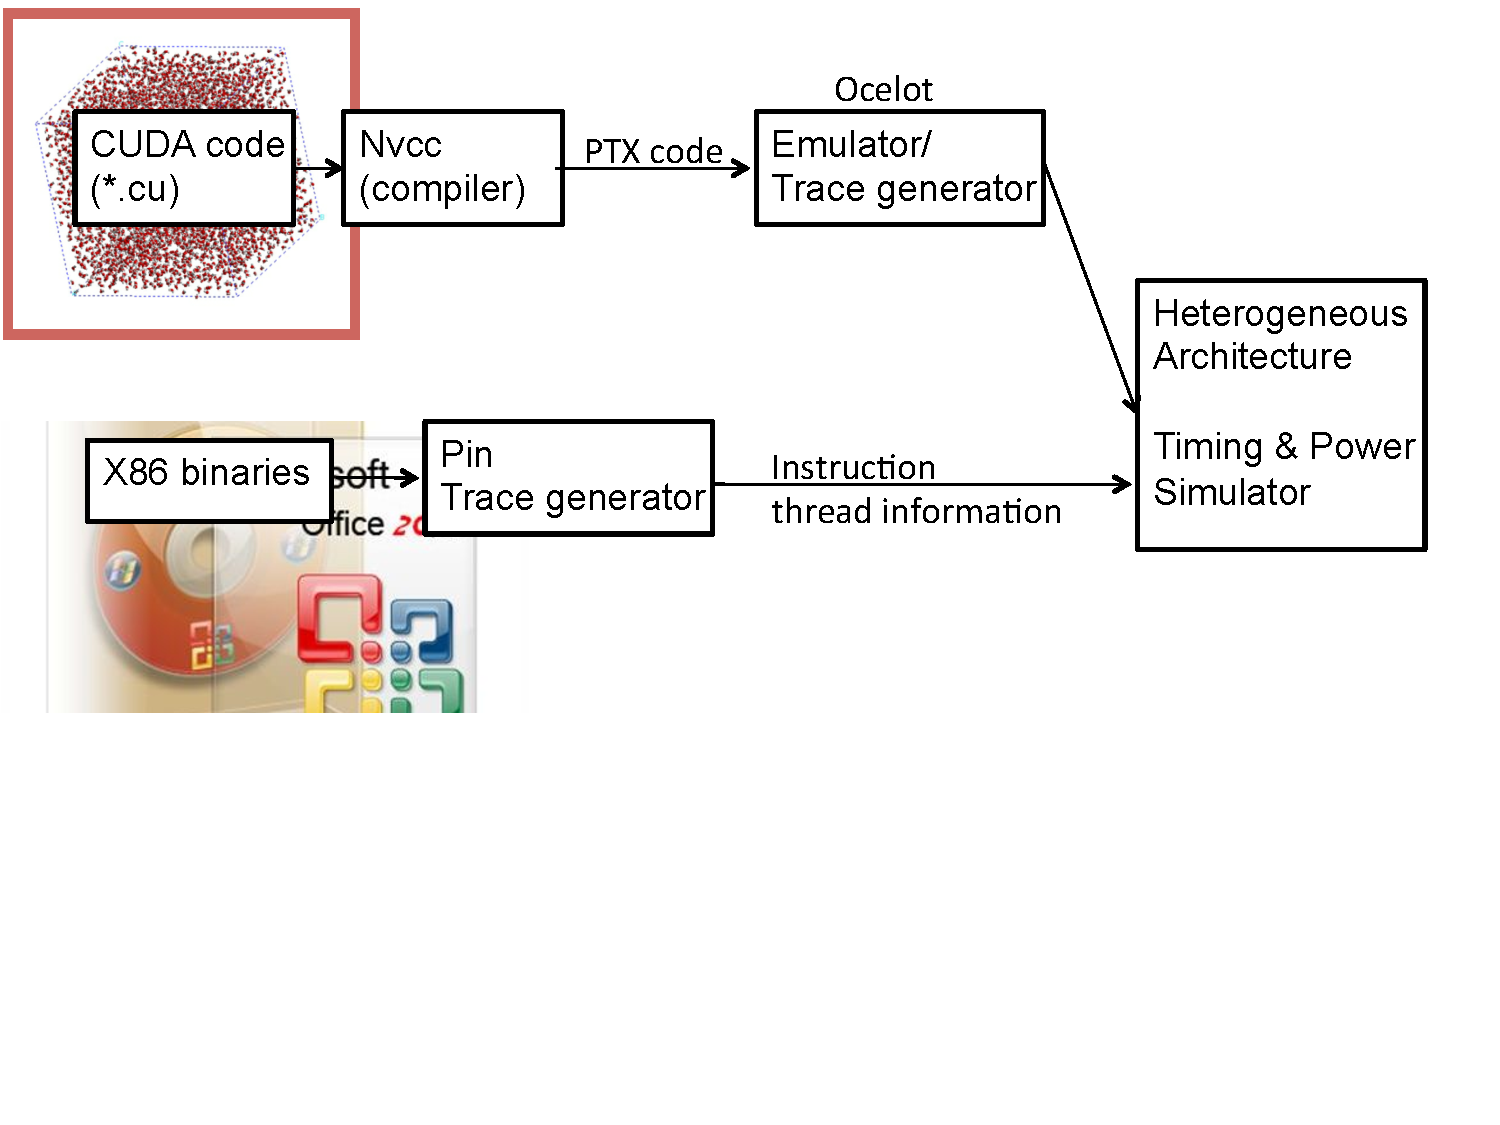
\includegraphics{figs/macsim_overview}
\caption{The overview of MacSim Simulator}
\label{fig:overview}
\end{figure*}

Figure~\ref{fig:overview} shows the overview of \SIM simulator.




%%%%%%%%%%%%%%%%%%%%%%%%%%%%%%%%%%%%%%%%%%%%%%%%%%%%%%%%%%%%%%%%%%%%%%%%
\section{Macsim Installation and Run}
%%%%%%%%%%%%%%%%%%%%%%%%%%%%%%%%%%%%%%%%%%%%%%%%%%%%%%%%%%%%%%%%%%%%%%%%


%%%%%%%%%%%%%%%%%%%%%%%%%%%%%%%%%%%%%%%%%%%%%%%%%%%%%%%%%%%%%%%%%%%%%%%%
\subsection{Download}
%%%%%%%%%%%%%%%%%%%%%%%%%%%%%%%%%%%%%%%%%%%%%%%%%%%%%%%%%%%%%%%%%%%%%%%%

\SIM source code is maintained using the subversion. 
You can check out the \SIM copy by


\begin{Verbatim}
svn co https://svn.research.cc.gatech.edu/macsim/trunk macsim-readonly --username readonly
\end{Verbatim}


%%%%%%%%%%%%%%%%%%%%%%%%%%%%%%%%%%%%%%%%%%%%%%%%%%%%%%%%%%%%%%%%%%%%%%%%
\subsection{Wiki and Other Supports}
%%%%%%%%%%%%%%%%%%%%%%%%%%%%%%%%%%%%%%%%%%%%%%%%%%%%%%%%%%%%%%%%%%%%%%%%

We manage the google project page in the following url: \url{http://code.google.com/p/macsim}


%%%%%%%%%%%%%%%%%%%%%%%%%%%%%%%%%%%%%%%%%%%%%%%%%%%%%%%%%%%%%%%%%%%%%%%%
\subsection{Build Requirement}
%%%%%%%%%%%%%%%%%%%%%%%%%%%%%%%%%%%%%%%%%%%%%%%%%%%%%%%%%%%%%%%%%%%%%%%%

\SIM requires following to build properly.

\begingroup
\renewcommand\descriptionlabel[1]{\textit{\hspace\labelsep{#1}}}
%\renewcommand\descriptionlabel[1]{\hspace\labelsep\cs{#1}}
\begin{description}\firmlist
  \item[Operating System] Currently, we only support linux
    distributions. Tested systems are as follows: \Verb+Ubuntu+, \Verb+Redhat (TODO)+.
  \item[Compiler] Any compiler that supports the C++0x (or C++11)
    standard library. Currently, we tested follwing compilers: \Verb+gcc+, \Verb+icc (TODO)+.
  \item[Autotools] - You need to have autotools (automake, autoconf,
    ...) version 2.65 or higher. You can install autotools by
\begin{Verbatim}
Ubuntu: apt-get install autotools-dev automake autoconf
Redhat: todo
\end{Verbatim}
\end{description}
\endgroup




\ignore{
\subsection{Directory Structure}

This section explains the directory structure of \SIM simulator.

\smallskip
\begin{lstlisting}
macsim/
  tag/ branch/ trunk/
\end{lstlisting}
\smallskip

\textit{Tag} directory has tagged version of \SIM
simulators. \textit{Branch} directory is for diverged \SIM, which is
currently empty. \textit{Trunk} directory is current working directory
for \SIM.

Following is more detailed information about \textit{Trunk} directory.

\smallskip
\begin{lstlisting}
trunk/
  bin/ def/ doc/ params/ scripts/ src/ tools/
\end{lstlisting}
\smallskip

\textit{Bin} directory contains the \SIM binary after the building
process. \textit{def} directory has knob (Section~\ref{sec:knob}) and
statistics (Section~\ref{sec:stat}) definitions. \textit{doc} has the
documentation. \textit{scripts} includes several scripts files that
are using during the building process. \textit{src} contains all
source files. \textit{tools} has several useful tools.
\ignore{ (Section~\ref{sec:tool}) }
}





%%%%%%%%%%%%%%%%%%%%%%%%%%%%%%%%%%%%%%%%%%%%%%%%%%%%%%%%%%%%%%%%%%%%%%%%
\subsection{Installation}
%%%%%%%%%%%%%%%%%%%%%%%%%%%%%%%%%%%%%%%%%%%%%%%%%%%%%%%%%%%%%%%%%%%%%%%%

The GNU Autotools (automake, autoconf) have been used for building
\SIM simulator. After initial check out of the \SIM copy, following commands are necessary.


\begin{Verbatim}
aclocal 
automake 
--add-missing 
autoconf 
./configure 
make
\end{Verbatim}

\noindent
You can combine above commands in a line:

\begin{Verbatim}
aclocal && automake --add-missing && autoconf && ./configure && make
\end{Verbatim}

\noindent
We provide autogen.sh script file to simplify the building process.

\begin{Verbatim}
./autogen.sh
make
\end{Verbatim}

The binary \textit{macsim} will be generated in the
\textit{trunk/bin/} directory.





%%%%%%%%%%%%%%%%%%%%%%%%%%%%%%%%%%%%%%%%%%%%%%%%%%%%%%%%%%%%%%%%%%%%%%%%
\subsection{Build Types}
%%%%%%%%%%%%%%%%%%%%%%%%%%%%%%%%%%%%%%%%%%%%%%%%%%%%%%%%%%%%%%%%%%%%%%%%

We provide three different build types.

\begin{itemize}
  \item opt : default, optimized version (-O3 flag)
  \item dbg : debug version (-g3 flag)
  \item gpf : gprof version (-pg flag)
\end{itemize}

\noindent
To build a certain type, you need to specify the option
after \textit{make} command. For example,

\begin{Verbatim}
make opt
make dbg
make gpf
\end{Verbatim}





%%%%%%%%%%%%%%%%%%%%%%%%%%%%%%%%%%%%%%%%%%%%%%%%%%%%%%%%%%%%%%%%%%%%%%%%
\subsection{How To Run \SIM}
%%%%%%%%%%%%%%%%%%%%%%%%%%%%%%%%%%%%%%%%%%%%%%%%%%%%%%%%%%%%%%%%%%%%%%%%

To run \textit{macsim} binary, two additional files are required in
the same directory.

\begin{itemize}
  \item params.in - defines architectural parameters that will
  overwrite the default value.

  \item trace\_file\_list - defines the number of traces to run and
  the path of each trace
\end{itemize}

%%%%%%%%%%%%%%%%%%%%%%%%%%%%%%%%%%%%%%%%%%%%%%%%%%%%%%%%%%%%%%%%%%%%%%%%
\subsubsection{params.in}
%%%%%%%%%%%%%%%%%%%%%%%%%%%%%%%%%%%%%%%%%%%%%%%%%%%%%%%%%%%%%%%%%%%%%%%%

We provide sample parameter files for various architectures (Intel
CPUs, NVIDIA GPUs, ...) in
the \textit{macsim-top/trunk/params}. Following is sample content of
params.in file.

\begin{Verbatim}
# Simulation Configuration
num_sim_cores 1
num_sim_small_cores 0
num_sim_medium_cores 0
num_sim_large_cores 1
core_type ptx
large_core_type x86
cpu_frequency 4
gpu_frequency 1.5
sim_cycle_count 0
max_insts 500000000
heartbeat_interval 1000000
forward_progress_limit 50000


# Common Core Configuration
fetch_policy rr
mt_no_fetch_br 1
one_cycle_exec 0
\end{Verbatim}

\noindent
The first literal is the name of parameter and the second literal is a
value that will overwrite the default value. Section~\ref{sec:knob}
details how to add, modify, and use these parameters.


%%%%%%%%%%%%%%%%%%%%%%%%%%%%%%%%%%%%%%%%%%%%%%%%%%%%%%%%%%%%%%%%%%%%%%%%
\subsubsection{trace\_file\_list}
\label{sec:trace_file_list}
%%%%%%%%%%%%%%%%%%%%%%%%%%%%%%%%%%%%%%%%%%%%%%%%%%%%%%%%%%%%%%%%%%%%%%%%

Following is the content of a sample trace\_file\_list.

\begin{Verbatim}
2
/trace/ptx/cuda2.2/FastWalshTransform/kernel_config.txt
/trace/ptx/cuda2.2/BlackScholes/kernel_config.txt
\end{Verbatim}

The first line is the number of traces that \SIM will run and
following lines are the path of each traces. Each top level trace
configuration file contains various information. Following is the
content of a top-level trace information file.


\begin{Verbatim}
1 x86
0 0
\end{Verbatim}

In the first line, the first number indicates the number of threads in
the application and second literal specifies the type of the
application. Trailing lines are the information of each thread
({thread id}, {thread starting point in terms of the instruction count
  of the main thread (thread 0)}). Section~\ref{sec:traceformat}
describes the detail of the trace file format.



%%%%%%%%%%%%%%%%%%%%%%%%%%%%%%%%%%%%%%%%%%%%%%%%%%%%%%%%%%%%%%%%%%%%%%%%
\subsubsection{Run}
%%%%%%%%%%%%%%%%%%%%%%%%%%%%%%%%%%%%%%%%%%%%%%%%%%%%%%%%%%%%%%%%%%%%%%%%

The following is the sample command lines to run \SIM simulator.

\begin{Verbatim}
./macsim [additional commands]
./macsim --l2_assoc=8 --stdout=stdout --stderr=stderr
./macsim --l1_assoc=4 
\end{Verbatim}


%%%%%%%%%%%%%%%%%%%%%%%%%%%%%%%%%%%%%%%%%%%%%%%%%%%%%%%%%%%%%%%%%%%%%%%%
\subsubsection{Repeating Trace}
%%%%%%%%%%%%%%%%%%%%%%%%%%%%%%%%%%%%%%%%%%%%%%%%%%%%%%%%%%%%%%%%%%%%%%%%

For multiple-application simulations, early terminated applications
sometimes need to be re-executed to model resource contention (cache,
on-chip interconnection, and memory controller) until all applications
finish. This is a common methodology to evaluate multi-program
workloads in the literature. \SIM also supports this feature. To
enable this feature, you need to

\begin{itemize}
  \item Specify the configuration in the command line by
  \begin{Verbatim}
  ./macsim --repeat_trace=1
  \end{Verbatim}

  \item Or you can write this in \textit{params.in} file
  \begin{Verbatim}
  repeat_trace 1
  \end{Verbatim}
\end{itemize}




%%%%%%%%%%%%%%%%%%%%%%%%%%%%%%%%%%%%%%%%%%%%%%%%%%%%%%%%%%%%%%%%%%%%%%%%
\section{Setting up Parameters}
\label{sec:parameter}
%%%%%%%%%%%%%%%%%%%%%%%%%%%%%%%%%%%%%%%%%%%%%%%%%%%%%%%%%%%%%%%%%%%%%%%%

This section provides sample examples for parameters to run different
types of simulations.



%%%%%%%%%%%%%%%%%%%%%%%%%%%%%%%%%%%%%%%%%%%%%%%%%%%%%%%%%%%%%%%%%%%%%%%%
\subsection{\cpu Experiments}
%%%%%%%%%%%%%%%%%%%%%%%%%%%%%%%%%%%%%%%%%%%%%%%%%%%%%%%%%%%%%%%%%%%%%%%%

%%%%%%%%%%%%%%%%%%%%%%%%%%%%%%%%%%%%%%%%%%%%%%%%%%%%%%%%%%%%%%%%%%%%%%%%
\subsubsection{One \cpu Core}
%%%%%%%%%%%%%%%%%%%%%%%%%%%%%%%%%%%%%%%%%%%%%%%%%%%%%%%%%%%%%%%%%%%%%%%%

Usually, we use large core configurations for specifying x86 cores
(however, it does not have to).

\begin{Verbatim}
// macsim-top/trunk/params/params_x86
num_sim_cores 1
num_sim_small_cores 0
num_sim_medium_cores 0
num_sim_large_cores 1
large_core_type x86
\end{Verbatim}


%%%%%%%%%%%%%%%%%%%%%%%%%%%%%%%%%%%%%%%%%%%%%%%%%%%%%%%%%%%%%%%%%%%%%%%%
\subsubsection{Multiple \cpu cores}
%%%%%%%%%%%%%%%%%%%%%%%%%%%%%%%%%%%%%%%%%%%%%%%%%%%%%%%%%%%%%%%%%%%%%%%%

Multiple core simulations are very similar to single core simulations,
but you need to specify the number of cores differently.


\begin{Verbatim}
// 4-core simulation
num_sim_cores 4
num_sim_small_cores 0
num_sim_medium_cores 0
num_sim_large_cores 4
large_core_type x86
repeat_trace 1
\end{Verbatim}


%%%%%%%%%%%%%%%%%%%%%%%%%%%%%%%%%%%%%%%%%%%%%%%%%%%%%%%%%%%%%%%%%%%%%%%%

\subsubsection{2-way SMT x86 Core}

\SIM also supports the simultaneous multi-threading (SMT) features.
These parameters are used for the SMT configurations:

\Verb+ max_threads_per_core+, \Verb+max_threads_per_medium_core+, and
\Verb+max_thread_per_large_core+. 

\noindent
For example,

\begin{Verbatim}
// 1-core 2-way SMT configuration
num_sim_cores 1
num_sim_small_cores 0
num_sim_medium_cores 0
num_sim_large_cores 1
large_core_type x86
max_threads_per_large_core 2
repeat_trace 1
\end{Verbatim}



%%%%%%%%%%%%%%%%%%%%%%%%%%%%%%%%%%%%%%%%%%%%%%%%%%%%%%%%%%%%%%%%%%%%%%%%
\subsection{\gpu Simulation}
%%%%%%%%%%%%%%%%%%%%%%%%%%%%%%%%%%%%%%%%%%%%%%%%%%%%%%%%%%%%%%%%%%%%%%%%

Usually, we use small core configurations for \gpu cores. We provide
several pre-defined configuration files for NVIDIA architectures. Here
are the list of sample files.

\begin{Verbatim}
params_8800gt // NVIDIA GeForce 8800GT (G80 architecture)
params_gtx280 // NVIDIA GeForce GTX280 (GT200 architecture)
params_gtx465, params_gtx480 // NVIDIA GeForece GTX465, GTX480 (Fermi architecture)
\end{Verbatim}


%%%%%%%%%%%%%%%%%%%%%%%%%%%%%%%%%%%%%%%%%%%%%%%%%%%%%%%%%%%%%%%%%%%%%%%%
\subsubsection{\gpu with One Application}
%%%%%%%%%%%%%%%%%%%%%%%%%%%%%%%%%%%%%%%%%%%%%%%%%%%%%%%%%%%%%%%%%%%%%%%%

\begin{Verbatim}
// 12-SM simulations
num_sim_cores 12
num_sim_small_cores 12
core_type ptx
max_threads_per_core 80 // set the max number of warps 
\end{Verbatim}


%%%%%%%%%%%%%%%%%%%%%%%%%%%%%%%%%%%%%%%%%%%%%%%%%%%%%%%%%%%%%%%%%%%%%%%%
\subsubsection{\gpu with Multiple Applications}
%%%%%%%%%%%%%%%%%%%%%%%%%%%%%%%%%%%%%%%%%%%%%%%%%%%%%%%%%%%%%%%%%%%%%%%%

\begin{Verbatim}
// 12-SM simulations, 6 SMs for each application
num_sim_cores 12
num_sim_small_cores 12
core_type ptx
max_threads_per_core 80 // set the max number of warps 
max_num_core_per_appl 6 // 6 SMs for each application
repeat_trace 1 // for multi-program workload simulation
\end{Verbatim}


%%%%%%%%%%%%%%%%%%%%%%%%%%%%%%%%%%%%%%%%%%%%%%%%%%%%%%%%%%%%%%%%%%%%%%%%
\subsection{Heterogeneous Simulation}
%%%%%%%%%%%%%%%%%%%%%%%%%%%%%%%%%%%%%%%%%%%%%%%%%%%%%%%%%%%%%%%%%%%%%%%%

For the CPU-GPU heterogeneous simulations, we model the architecture
similar to Intel's Sandy Bridge~\cite{sandybridge}. However, we
model \gpu cores similar to NVIDIA Fermi~\cite{fermi} architecture. We
also provide sample files for the heterogeneous simulations.

\begin{Verbatim}
params_hetero_1_6 // 1-CPU, 6-GPU cores
params_hetero_4c_4g // 4-CPU, 4-GPU cores
\end{Verbatim}


%%%%%%%%%%%%%%%%%%%%%%%%%%%%%%%%%%%%%%%%%%%%%%%%%%%%%%%%%%%%%%%%%%%%%%%%
\subsubsection{One CPU application + One GPU application}
%%%%%%%%%%%%%%%%%%%%%%%%%%%%%%%%%%%%%%%%%%%%%%%%%%%%%%%%%%%%%%%%%%%%%%%%

Following example shows simple heterogeneous configuration.

\begin{Verbatim}
num_sim_cores 2
num_sim_small_cores 1
num_sim_medium_cores 0
num_sim_large_cores 1
core_type ptx
large_core_type x86
cpu_frequency 3
gpu_frequency 1.5
repeat_trace 1
\end{Verbatim}


Although above configurations set up the number of CPU and GPU cores
correctly, you need to setup each core types individually. Please
refer to sample files.

%%%%%%%%%%%%%%%%%%%%%%%%%%%%%%%%%%%%%%%%%%%%%%%%%%%%%%%%%%%%%%%%%%%%%%%%
\subsubsection{Multiple CPU applications + Multiple GPU applications}
%%%%%%%%%%%%%%%%%%%%%%%%%%%%%%%%%%%%%%%%%%%%%%%%%%%%%%%%%%%%%%%%%%%%%%%%

\begin{Verbatim}
num_sim_cores 8
num_sim_small_cores 4
num_sim_medium_cores 0
num_sim_large_cores 4
core_type ptx
large_core_type x86
cpu_frequency 3
gpu_frequency 1.5
repeat_trace 1
\end{Verbatim}


%%%%%%%%%%%%%%%%%%%%%%%%%%%%%%%%%%%%%%%%%%%%%%%%%%%%%%%%%%%%%%%%%%%%%%%%
\subsection{Micro-architecture configuration}
%%%%%%%%%%%%%%%%%%%%%%%%%%%%%%%%%%%%%%%%%%%%%%%%%%%%%%%%%%%%%%%%%%%%%%%%

%%%%%%%%%%%%%%%%%%%%%%%%%%%%%%%%%%%%%%%%%%%%%%%%%%%%%%%%%%%%%%%%%%%%%%%%
\subsubsection{Number of Thread Blocks Per Core}
%%%%%%%%%%%%%%%%%%%%%%%%%%%%%%%%%%%%%%%%%%%%%%%%%%%%%%%%%%%%%%%%%%%%%%%%

The Maximum number blocks per core will be determined by several
factors: 1) the number of threads per thread block, 2) the number of
register used, 3) the number of shared memory usage, and 4) NVIDIA
CUDA computing version. NVIDIA provides the occupancy calculator to
get the number. \SIM uses this value to allocate a number of thread
blocks in each core. Since this value is per-application
characteristic, it is not possible to use single value nor provide the
value individually. Instead, our approach is that using information
provided by GPUOcelot~\cite{ocelot} while generating traces. This
information is written in the trace file and \SIM uses it. However, we
also provide a way to override the value by
setting \Verb+max_block_per_core_super+.



%%%%%%%%%%%%%%%%%%%%%%%%%%%%%%%%%%%%%%%%%%%%%%%%%%%%%%%%%%%%%%%%%%%%%%%%
\subsubsection{Cache Configuration}
%%%%%%%%%%%%%%%%%%%%%%%%%%%%%%%%%%%%%%%%%%%%%%%%%%%%%%%%%%%%%%%%%%%%%%%%

The cache can be configured by following parameters.

\begin{Verbatim}
l{1,2}_{small, medium, large}_num_set // number of sets
l{1,2}_{small, medium, large}_assoc // associativity
l{1,2}_{small, medium, large}_line_size // cache line size
l{1,2}_{small, medium, large}_num_bank // number of banks  
l{1,2}_{small, medium, large}_latency // cache latency
l{1,2}_{small, medium, large}_bypass // cache bypass (if set, always miss)
num_l3 // number of l3 cache tiles
l3_num_Set // number of l3 cache sets
l3_assoc // l3 associativity
l3_line_size // l3 line size
l3_num_bank // l3 number of banks
l3_latency // l3 latency
l{1,2,3}_{read,write}_port // the number of read / write port
icache_num_set  8 // 4KB I-cache 
icache_assoc   8 // I cache set associativity 
\end{Verbatim}


The effective cache size can be calculated by the
Equation~\ref{eq:cachesize}.

\begin{equation}
\label{eq:cachesize}
cache\_size = num\_set \times assoc \times line\_size \times num\_tiles (l3 only, otherwise 1)
\end{equation}


\noindent
For example, to configure a 16-way 1MB cache with 64B line size,

\Verb+ 1MB cache = 256 sets * 16 way *+ \Verb+64B * 4 tiles+
%\Verb+\textsf{16 way} $\times$ \textsf{64 B}+ $\times$
%\Verb+\textsf{4 tiles}+. 

\noindent
Also, the cache latency is determined by several factors including the
size, technology, and the number of ports. Cacti~\cite{cacti} can be
used to model accurate cache latency. The cache line size is set as
64B by default. Although the cache line size can be any power of 2,
all cache levels should have the same size.


%%%%%%%%%%%%%%%%%%%%%%%%%%%%%%%%%%%%%%%%%%%%%%%%%%%%%%%%%%%%%%%%%%%%%%%%
\subsubsection{DRAM configuration}
\label{sec:param-dram}
%%%%%%%%%%%%%%%%%%%%%%%%%%%%%%%%%%%%%%%%%%%%%%%%%%%%%%%%%%%%%%%%%%%%%%%%

We model three key components in the memory scheduler: timing
constraints, bandwidth, and scheduling policy. Following are key
parameters used in the \SIM.


\begin{Verbatim}
dram_frequency 0.8 // dram frequency
dram_bus_width 4 // dram bus width
dram_column 11 // column access (CL) latency
dram_activate 25 // row activate (RCD) latency
dram_precharge 10 // precharge (RP) latency
dram_num_mc 2 // number of memory controllers
dram_num_banks 8 // number of banks per controller
dram_num_channel 2 // number of dram channels per controller
dram_rowbuffer_size 2048 // row buffer size
dram_scheduling_policy FRFCFS // dram scheduling policy
\end{Verbatim}


Dram timings using three parameters: precharge ($t_{RP}$), activate
($t_{RCD}$), and column access ($t_{CL}$) latency. DRAM bandwidth is
modeled using three
parameters: \Verb+dram_frequency+, \Verb+dram_bus_width+,
and \Verb+dram_num_channel+. The maximum DRAM bandwidth can be
calculated using Equation~\ref{eq:bandwidth}.

\begin{equation}
\label{eq:bandwidth}
max\_bandwidth = dram\_frequency \times dram\_bus\_width \times dram\_num\_mc \times dram\_num\_channel 
\end{equation}

For example, the maximum bandwidth from above parameters can be
\Verb+ 800 MHz (0.8 GHz)} * 4 Bytes+
  \Verb+* 2 MCs * 2 Channels = 12.8GB/s+ . Finally, \SIM provides
  multiple DRAM scheduling policies: FCFS (First-Come-First-Serve) and
  FR-FCFS (First-Ready First-Come-First-Serve).


%%%%%%%%%%%%%%%%%%%%%%%%%%%%%%%%%%%%%%%%%%%%%%%%%%%%%%%%%%%%%%%%%%%%%%%%
\subsubsection{Setting \cpu Core Parameters}
%%%%%%%%%%%%%%%%%%%%%%%%%%%%%%%%%%%%%%%%%%%%%%%%%%%%%%%%%%%%%%%%%%%%%%%%

By default these configurations are applied to small cores. 

\begin{Verbatim}
width   2 // pipeline width (the entire pipelines use the same width) 
fetch_latency 5 // front-end depth 
alloc_latency 5 // decode/allocation depth  
bp_dir_mech   gshare 
bp_hist_length 14 // branch history length 
isched_rate 4  // # of integer instructions that can be executed per cycle 
msched_rate 2  // # of memory instructions that can be executed per cycle 
fsched_rate  2  // # of FP instructions that can be executed per cycle 
schedule  io, ooo // instruction scheduling policy 
rob_size    96  // ROB size
fetch_policy rr // SMT(MT) thread fetch policy  by default: round-robin 
\end{Verbatim}


%%%%%%%%%%%%%%%%%%%%%%%%%%%%%%%%%%%%%%%%%%%%%%%%%%%%%%%%%%%%%%%%%%%%%%%%
\subsubsection{Setting GPU Core Parameters}
%%%%%%%%%%%%%%%%%%%%%%%%%%%%%%%%%%%%%%%%%%%%%%%%%%%%%%%%%%%%%%%%%%%%%%%%
{\textbf GPU Core Parameters} 

\TODO{Question: is constant cache size is per SM? How does a core share the constant cache, texture cache, what is ptx\_exec\_ratio? } 


\begin{Verbatim}
schedule_ratio 4 \\ Every 4th cycle, one thread (warp) is scheduled 
fetch_ratio  4 \\ Every 4th cycle, one thread (warp) is fetched 
gpu_sched   1 \\ set GPU scheduler 
ptx_common_cache \\ 
const_cache_size  1024 \\ 1024B constant cache  
texture_cache_size 1024  \\ 1024B texture cache
shared_mem_size 4096  \\ 4096B shared memory size 
ptx_exec_ratio  \\ 
num_warp_scheduler \\ the number of warps (threads) can be scheduled  
\end{Verbatim}








\ignore{
\subsubsection{Hardware Prefetching}

We provide stride hardware prefetcher~\cite{iac:spr04}. 
}



% LocalWords:  Macsim MacSim NVIDIA PTX multicore RISC uops microarchitecture
% LocalWords:  NoC SMT McPat
